\documentclass[12pt,twoside]{article}

% *** Set page dimensions ***
\raggedbottom
\parindent=0in
%\setlength{\topmargin}{-0.5in}
%\setlength{\oddsidemargin}{0.1875in}
%\setlength{\evensidemargin}{0in}
%\setlength{\textheight}{8.5in}
%\setlength{\textwidth}{6.225in}
%\addtolength{\oddsidemargin}{-0.7in}
%\addtolength{\evensidemargin}{-1.2in}
%\setlength{\oddsidemargin}{-0.2in}
%\setlength{\evensidemargin}{-0.2in}
%\addtolength{\textwidth}{1.4in}
%\addtolength{\topmargin}{-.875in}
%\addtolength{\textheight}{2.00in}

% *** Packages ***
\usepackage{alltt}
\usepackage{tocloft}
\usepackage{graphicx}
\usepackage{lscape}
\usepackage{amssymb}
\usepackage{float}
\usepackage{amsmath}
\usepackage{gensymb}
%\usepackage{subfigure}
\usepackage{lscape}
\usepackage{epsfig}
\usepackage{enumerate}
\usepackage{multicol}
\usepackage{fancyhdr}
\usepackage{epstopdf}
\usepackage{hyperref}
\usepackage{listings}

% *** Table of contents and Sectioning *** 
\setcounter{secnumdepth}{0}
\setcounter{tocdepth}{5}

% *** Table of contents and Sectioning *** 
\newcommand{\next}{\addtocounter{enumi}{9} \item}
\newcommand{\now}[1]{\setcounter{enumi}{#1}}
\newcommand{\Z}{\mbox{\sf Z\hspace{-1.5mm}Z}}
\newcommand{\R}{\mbox{\rm I\hspace{-0.75mm}R}}
\columnsep=0.75in

% *** Shortcuts for syntax ***
\newcommand{\ds}{\displaystyle }
\newcommand{\vsc}{\vspace{4mm}}
\newcommand{\dd}[1]{\frac{d}{d{#1}} \,} 
\newcommand{\ddx}{\frac{d}{dx} \,} 
\newcommand{\ddy}{\frac{d}{dy} \,} 
\newcommand{\ddz}{\frac{d}{dz} \,} 
\newcommand{\dydx}{\frac{dy}{dx} \,} 
\newcommand{\dydt}{\frac{dy}{dt} \,} 
\newcommand{\dfdx}{\frac{df}{dx} \,} 
\newcommand{\ddt}[1]{  \frac{d{#1}}{dt} }
\newcommand{\pp}[2]{  \frac{\partial{#1}}{\partial {#2}} }
\newcommand{\zx}{\frac{\partial z}{\partial x} \,}
\newcommand{\zy}{\frac{\partial z}{\partial y} \,}
\newcommand{\limh}{\lim_{h \rightarrow 0} \;}
\newcommand{\diff}{\frac{d}{dx} \,}
\newcommand{\de}{\Delta}
\renewcommand{\thesection}{\Roman{section}}
\newcommand{\bfr}{\begin{flushright}}
\newcommand{\efr}{\end{flushright}}
\newcommand{\dx}{\frac{\partial f}{\partial x} \,}
\newcommand{\dy}{\frac{\partial f}{\partial y} \,}
\newcommand{\p}{\partial}
\newcommand{\vi}{\vec{i}}
\newcommand{\vj}{\vec{j}}
\newcommand{\vk}{\vec{k}}
\newcommand{\lan}{\left\langle}
\newcommand{\ran}{\right\rangle}
\newcommand{\reading}[1] { {\em Reading: #1}}
\renewcommand{\Pr}{ \mbox{Pr}}

% *** Commands related to textbook references
\newcommand{\problem}{{\bf Problem.} }

% *** Footnoting with symbols ***
\long\def\symbolfootnote[#1]#2{\begingroup%
\def\thefootnote{\fnsymbol{footnote}}\footnote[#1]{#2}\endgroup}

% *** Defining a boxed note ***
\floatstyle{boxed}
\newfloat{noteinbox}{htb}{loa}
\newenvironment{boxnote}{\begin{noteinbox}[H]}{\end{noteinbox}}

\newcommand{\Question}{ {\bf Question: }  }
\newcommand{\Example}[1]{ {\bf Example: } {\em #1} }
\newcommand{\ExampleCont}[1]{ {\em #1} }

% *** Define the boxed Week #/summary at the beginning/end of every chapter ***
\newcommand{\sectionbox}[1]{% 
\begin{tabular}{|p{6in}|}%
\hline%
\ \\ %
{\Large {\bf {#1}}}  \\%
\ \\%
\hline%
\end{tabular}}

% *** Shortcuts *** 
\newcommand\goals{\large {\bf {Goals:}}}
\newcommand\setfont{ }

% *** Week commands: overwritten in each notes file
\newcommand{\Week}{Null-InPreambleCommon}
\newcommand{\WeekTitle}{Null-InPreambleCommon}
\newcommand{\Course}{MNTC P04}
\newcommand{\SetNum}{1 }
\newcommand{\topic}[1]{
\newpage
\setcounter{page}{1}
\fancyhead[LE,RO]{#1 - \thepage}
}

% *** Setup Latex for the large version of the files ***
%\usepackage[landscape]{geometry}
\usepackage[letterpaper,landscape,hmargin={.8in,.8in},vmargin={1in,0.2in}]{geometry}

% Remove paragraph indents
\setlength{\parindent}{0pt}

% Spacing at the top for the header is too large by default
\setlength{\voffset}{-5ex}

% **** RENEW SCALING COMMANDS HERE ****
% *** Text in boxes ***
\renewenvironment{boxnote}{\begin{noteinbox}[H] \huge}{\end{noteinbox}} 

% *** Chapter lead in/summary boxes ***
\renewcommand{\sectionbox}[1]{% 
\begin{tabular}{|p{9.5in}|}%
\hline%
\ \\ %
{\huge {\bf {#1}}}  \\%
\ \\%
\hline%
\end{tabular}}

% *** 'Section'' commands, which are sometimes used for spacing
% From http://zoonek.free.fr/LaTeX/LaTeX_samples_section/0.html
\makeatletter
 \renewcommand\section{\@startsection {section}{1}{\z@}%
                                    {-3.5ex \@plus -1ex \@minus -.2ex}%
                                    {0.3ex \@plus.2ex}%
                                    {\setfont\bf}}

 \renewcommand\subsection{\@startsection {subsection}{1}{\z@}%
                                    {-3.5ex \@plus -1ex \@minus -.2ex}%
                                    {0.3ex \@plus.2ex}%
                                    {\setfont\bf}}

% *** 'Goals' should be larger in the overheads ***
\renewcommand\goals{\huge {\bf {Goals:}}}
\renewcommand\setfont{\huge }

\thispagestyle{empty}

\setfont 

\newcommand{\WeekTitleOne}{Derivatives - Foundations}
\newcommand{\WeekTitleTwo}{Derivatives - Linearization and Applications}
\newcommand{\WeekTitleThree}{Derivatives - Modeling}
\newcommand{\WeekTitleFour}{Integrals - Foundations}
\newcommand{\WeekTitleFive}{Integrals - Techniques}
\newcommand{\WeekTitleSix}{Integrals - Modeling}
\newcommand{\WeekTitleSeven}{Differential Equations - }
\newcommand{\WeekTitleEight}{Differential Equations - }
\newcommand{\WeekTitleNine}{Differential Equations - }
\newcommand{\WeekTitleTen}{Linear Algebra - }
\newcommand{\WeekTitleEleven}{Linear Algebra - }
\newcommand{\WeekTitleTwelve}{Linear Algebra - }



\newcommand{\Fe}{ F_{\mbox{ext}} }

\begin{document}
\setfont
\pagestyle{fancy}
\renewcommand{\Week}{8 }
\renewcommand{\WeekTitle}{\WeekTitleEight }

\fancyhead[LE,RO]{Week \Week}  % default, usually only for first page
\fancyfoot{}
\sectionbox{Week \#\Week: \WeekTitle}

\vspace{5mm}
\goals
\begin{itemize}
\item Express real world situations in terms of second order linear
  differential equations.
\item Describe the difference between homogeneous and nonhomogeneous
  second order linear differential equations.
\item Use MATLAB to solve linear and nonlinear second order
  differential equations, both homogeneous and nonhomogeneous.
\end{itemize}
\vspace{5mm}

\newpage

\topic{Second-Order Linear Equations - Spring System Intro}
\section*{Second-Order Linear Equations - Spring System}

So far we have seen examples of {\bf first-order DEs}, or equations
with first derivatives of some unknown function.  

From here on in the course, we will study differential equations with
{\bf second or higher derivatives}.

One classic source of differential equations of this type comes from 
analyzing the forces on a block at the end of a spring.
\begin{center}
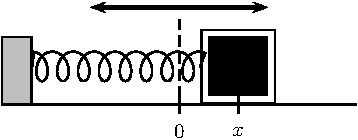
\includegraphics[width=0.5\linewidth]{graphics/notes_08_block}
\end{center}


While the mathematics behind this simple system will be very
interesting in their own right, we should also note at the outset that
the simple spring/mass model can be applied to a wide variety of
not-so-obviously related real-world problems.

\begin{center}
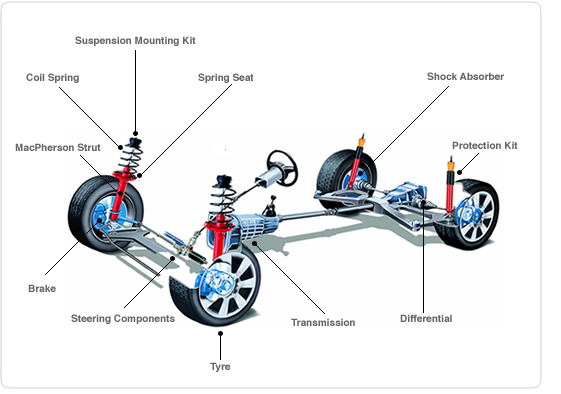
\includegraphics[width=0.30\linewidth]{graphics/notes_08_SpringSystemCar}
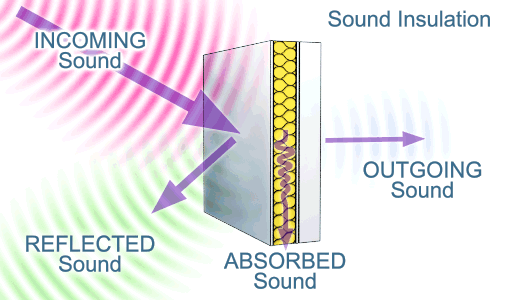
\includegraphics[width=0.30\linewidth]{graphics/notes_08_Sound-Attenuation} \\
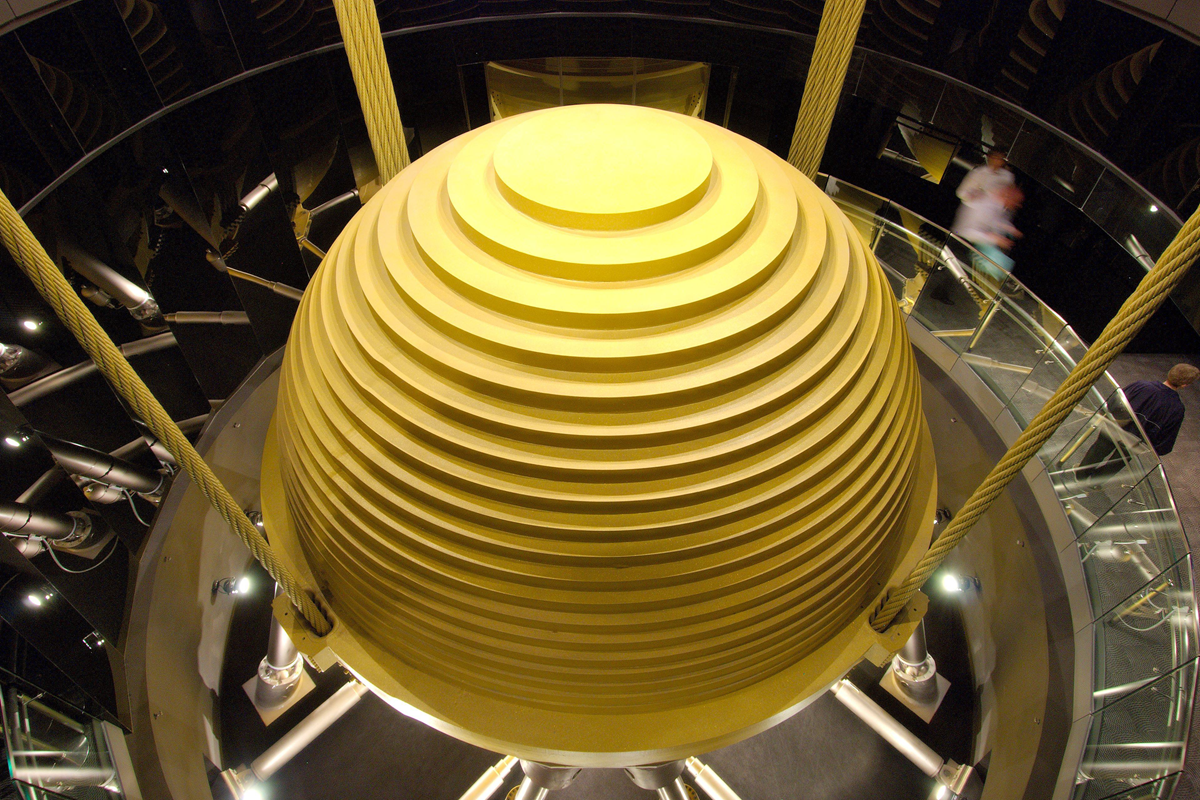
\includegraphics[width=0.30\linewidth]{graphics/notes_08_Tuned_Mass_Damper_atop_Taipei_101_-_27_March_2008}
\end{center}

\newpage

\topic{Spring System Analysis}
\subsection*{Spring System Analysis}

\begin{center}
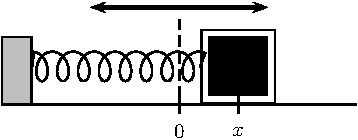
\includegraphics[width=0.5\linewidth]{graphics/notes_08_block}
\end{center}

In this system, how would you describe $x$ in words?

\newpage
\problem Draw a free-body diagram for the mass.  Indicate the magnitude of the forces, assuming 
\begin{itemize}
\item the mass of the block is $m$ kg, and
\item the spring constant (in $N/m$) is
  given by the constant $k$.
\end{itemize}

\newpage
Let us work with our intuition about this system before beginning the mathematics.

If the spring is very stiff, is $k$ large or small?
\vfill

\newpage
{\bf Period}: the length of time to complete one full cycle/oscillation.
\vspace{0.2in}

If we increase the stiffness of the spring, do you expect the {\em period} 
of the oscillations to increase or decrease?  Why?

\vfill

If we increase the mass, do you expect
the \emph{period} of the oscillations to increase or decrease? Why?

\vfill

\newpage

If we know $k$ and $m$, and assume that friction is negligible, should
we be able to determine the exact period of the oscillations?  \vfill


\vfill

From the work so far, can we easily find the formula for the period?

\vfill

\newpage

The spring system is an excellent introduction to higher-order differential equations because 
\begin{itemize}
\item we all have an intuition about how it \emph{should} work physically,
\item the mathematics and physics are simple, and
\item there's no obvious way to predict critical features (e.g. the
  period) from the given information.
\end{itemize}
We clearly need some new tools!

\newpage
\topic{Spring System as a DE}
\subsection*{Spring System as a DE}

Use Newton's second law, $F = ma$, to construct an equation involving
the position $x(t)$.  \vfill

What order of differential equation does $F=ma$ produce for this
spring/mass system?

\vfill

\newpage

To simplify matters temporarily, let us assume that both
  $k = 1 $ N/m and $m = 1$ kg. Rewrite the previous differential
  equation.
\vfill

This differential equation invites us to find a function $x(t)$ whose
second derivative is its own negative.  What function(s) would satisfy
that?  \vfill

\newpage

Having found two (and more) solutions to the differential equation for
the spring/mass system

\newpage

\topic{Classifying Second-Order DEs}
\subsection*{Classifying Second-Order DEs}

% The generic 2nd order DE with constant coefficients is of the form 
% $$a y'' + b y ' + cy = 0$$
% where $a, b, c \in \RR$.

 Classify the following DEs based on the terms {\em homogeneous}, {\em linear} and {\em constant coefficients}
 \vfill
 $x^2 y'' +  x y' + y = 10$
 \vfill

 $ 100 y'' +  y = 4x^3$
 \vfill

 $ (y'')^2 + y = 4 e^{x}$
 \vfill

 $ 4 y'' - 10 y' + y = 0 $
 \vfill

 \newpage


\topic{Mechanical Vibrations - Spring-mass system}
\section*{Mechanical Vibrations - Spring-mass system}

We now consider the spring/mass system seen earlier, but with more
detail.

Consider a mass $m$ hanging on the end of a vertical spring of
unstretched length $\ell$.  Using Newton's second law, build a
differential equation that governs the system.

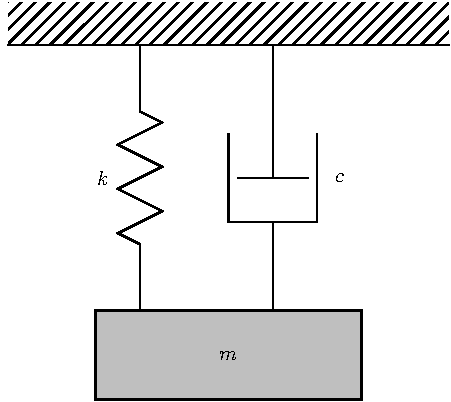
\includegraphics[width=0.4\linewidth]{graphics/notes_08_hanging_mass}

\newpage

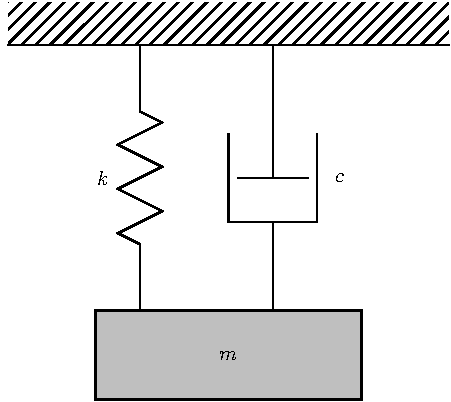
\includegraphics[width=0.4\linewidth]{graphics/notes_08_hanging_mass}


% \begin{itemize}
% \item Gravity acts downward and has a magnitude of $mg$ where $g$ is the
%   acceleration due to gravity; $F_g = mg$.
% \item The spring acts upward and, by Hooke's law, has a magnitude proportional
%   elongation.  If $y$ represents the displacement of the mass from the
%   equilibrium position, then $F_s = -k(\ell +y)$.
% \item Assuming that possible damping forces (i.e.\ a dashpot) are directly
%   proportional to the velocity of the mass, we have $F_d = - cy'$.
% \item There may be an external driving force $F(t)$.
% \end{itemize}
% Summing the forces, we find that $m y'' = F_g + F_s + F_d + F(t) = mg -k(\ell
% +y) -cy' + F(t)$.  At equilibrium, we have $mg = k\ell$ so the standard form of
% the equation is
% \[
% y'' + \tfrac{c}{m} y' + \tfrac{k}{m} y = \tfrac{1}{m} F(t) \, . 
% \]


\newpage
\problem  Consider a mass of $0.5 \; \text{kg}$ with spring constant $k = 2 \; \text{N}
  \cdot \text{m}^{-1}$ in an undamped unforced system.  Assume the mass is
  displaced $0.4 \; \text{m}$ from equilibrium and released.  Describe the
  long-term behaviour of the system.

\newpage
\topic{Unforced Spring/Mass System - Patterns of Behaviour}
\subsection*{Unforced Spring/Mass System - Patterns of Behaviour}

\begin{center}
\begin{minipage}{0.35\linewidth}
\vspace{0pt}
\begin{center}
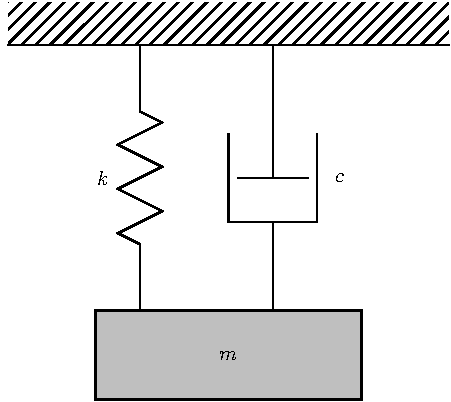
\includegraphics[width=0.5\linewidth]{graphics/notes_08_hanging_mass}
$m y'' =  -k y - c y'$ \\
or
$$my'' + cy' + ky =  0$$ \\[2ex]

$$r = \frac{-c \pm \sqrt{c^2 - 4 km}}{2m}$$
\end{center}
\end{minipage}
\begin{minipage}{0.6\linewidth}
\vspace{0pt}
\begin{tabular}{|c|c|c|c|} \hline
Damping  & $\quad c^2 - 4km \quad$ & $\; \quad r\quad\;$ & Description \\ \hline
None & & & \\[1ex]  
$c=0$ & & & \\[1ex]   \hline
Light & & & \\[1ex]  
$c^2 < 4km$ & & & \\[1ex]   \hline
 & & & \\[1ex]  
& & & \\[1ex]   \hline
Heavy & & & \\[1ex]  
$c^2 > 4km$ & & & \\[1ex]   \hline
\end{tabular}
\end{minipage}
\end{center}

\newpage

\problem Sketch possible solutions for all four spring/mass cases.
  \begin{minipage}[h]{0.475\linewidth}
    \begin{center}
      
   \vspace{0pt} 
   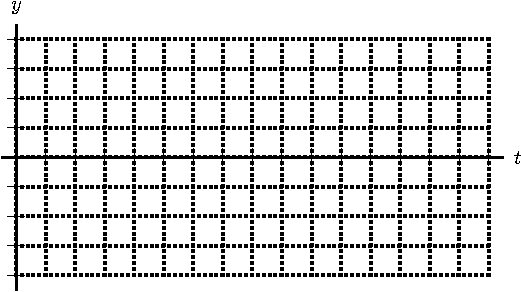
\includegraphics[width=0.5\linewidth]{graphics/notes_08_spring_mass_axes}\\
Undamped 

\hrulefill

   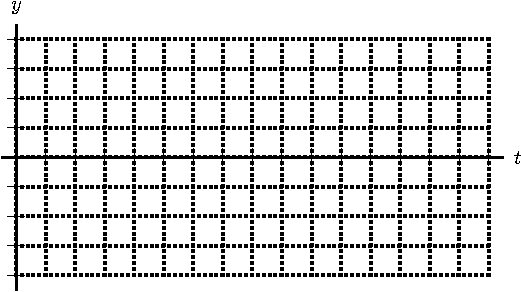
\includegraphics[width=0.5\linewidth]{graphics/notes_08_spring_mass_axes}\\
Critically Damped
    \end{center}
  \end{minipage}
  \begin{minipage}[h]{0.475\linewidth}
    \begin{center}
      
   \vspace{0pt} 
   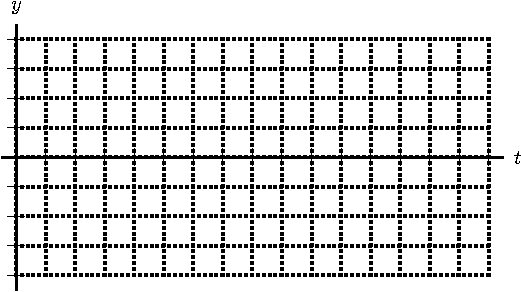
\includegraphics[width=0.5\linewidth]{graphics/notes_08_spring_mass_axes}\\
Damped  

\hrulefill

   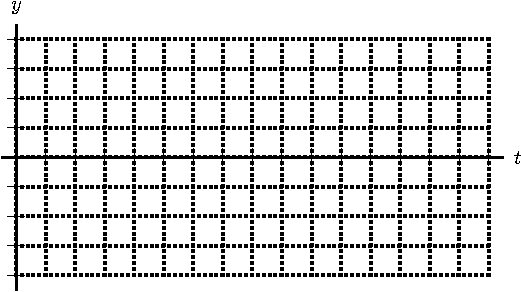
\includegraphics[width=0.5\linewidth]{graphics/notes_08_spring_mass_axes}\\
Overdamped
    \end{center}
  \end{minipage}


% \begin{remark}
%   If we have $c^2 > 4km$, then the system is \define{overdamped}.  In
%   this case, the general solution is $y(t) = C_1 e^{r_1 t} + C_2
%   e^{r_2 t}$ where $r_{1,2} = \frac{-c \pm \sqrt{c^2 -4km}}{2m}$.  The
%   friction/damping is strong in comparison with a relatively weak
%   spring or a small mass.  The mass settles to its equilibrium
%   position with out any oscillations.
% \end{remark}

% \vfill

% \newpage

% \begin{remark}
%   If we have $c^2 = 4km$, then the system is \define{critically damped}.  In
%   this case, the general solution is $y(t) = (C_1 + C_2 t) e^{r t}$ where $r =
%   \frac{-c}{2m}$.  The resistance is just large enough to damp out any
%   oscillations. \comment{Ideally, a door-closer is critically damped.}
% \end{remark}

\newpage

\topic{Demonstration - Spring/Mass}
\section*{Demonstration - Spring/Mass}

We will demonstrate how the solutions to the damped spring/mass DE
change as the damping is gradually increased.  

$$m y'' + c y' + k y  = 0$$

In this demonstration, we will use $m = 1$ kg, and $k = 25$ N/m.

\newpage

$$y'' + c y' + 25 y  = 0$$      \\[1ex]
\problem
  What damping level will produce {\em critical damping}?
\vfill

  What will the form of the solutions be when damping is {\bf below} critical?

\vfill
  What will the form of the solutions be when damping is {\bf above} critical?
\vfill
\newpage

During demonstration, try to ask yourself the following questions:
\begin{itemize}
\item As damping increases in general, does the {\bf graph} of the
  solution change gradually or dramatically?  \\What about the {\bf
    mathematical form} of the solution?
\item Near critical damping specifically, does the {\bf graph} of the
  solution change gradually or dramatically?  \\What about the {\bf
    mathematical form} of the solution?
\end{itemize}


\newpage
\topic{Applications - Pendulum }
\section*{Applications - Pendulum }
\problem
Consider the simple pendulum (mass at the end of a rod) shown below.
\begin{center}
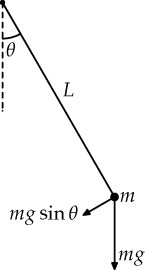
\includegraphics[height=2.5in]{graphics/notes_08_Simple-Pendulum-Labeled-Diagram}
\end{center}

If we start from the rotational (torque) version of Newton's Second Law,
 
\begin{center}
  (moment of inertia) $\cdot$ (angular accel) = $\ds \sum $ torques \\ 
we obtain \\
$(m L^2) \cdot ( \theta '') = -mg L \sin(\theta)$ \\
or, in (almost) standard form: 
\end{center}

\newpage
$$ \theta'' + \frac{g}{L} \sin(\theta) = 0$$

Use a well-known approximation from calculus to simplify this to a
linear DE:

\vfill

What limitations does this put on our interpretation of the solution?

\vfill

\newpage

Find the general solution to the linearized differential equation
$$ \theta'' + \frac{g}{L} \theta = 0$$

\vfill

Use your solution to predict the period of the oscillations of a
pendulum, given $g$ and the length of the rod, $L$.

\vfill

\newpage

Comment: what does this mean about the swinging of a pendulum for
larger angles?


\newpage
\topic{Nonhomogeneous Linear Differential Equations - Theory}
\section*{Nonhomogeneous Linear Differential Equations}

In the previous lectures, we have learned how to solve linear DEs with
constant coefficients.  Any degree was fine, but the equations had to
be {\bf homogeneous}: \\[2ex]
$$ y^{(n)} + a_{n-1} y^{(n-1)} + a_{n-2} y^{(n-2)} + \ldots + a_1 y' + a_0 y = 0$$ \\[2ex]


This week, we explore how to deal with equations with more interesting
right-hand sides.

% \newpage
% \begin{proposition}
%   If $y_1(x)$ and $y_2(x)$ are solutions of the \emph{nonhomogeneous} equation
%   \[
%   y'' + p(x) y' + q(x) y = f(x) \, ,
%   \] 
%   then $y_1(x) - y_2(x)$ is a solution to the
%   homogeneous equation $$y'' + p(x) y' + q(x) y = 0$$
% \end{proposition}

% Prove this. 

% \begin{proof}
%   Linearity yields
%   \begin{align*}
%     \Bigl( \tfrac{d^2}{dx^2} + p(x) \tfrac{d}{dx} + q(x) \Bigr) \bigl( y_1 -
%     y_2 \bigr) &= \Bigl( \tfrac{d^2}{dx^2} + p(x) \tfrac{d}{dx} + q(x) \Bigr)
%     \bigl( y_1 \bigr) - \Bigl( \tfrac{d^2}{dx^2} + p(x) \tfrac{d}{dx} + q(x)
%     \Bigr) \bigl( y_2 \bigr) \\
%     &= f(x) - f(x) = 0 \, \qedhere
%   \end{align*}
% \end{proof}

\vfill

\newpage

  The general solution of a nonhomogeneous $n$-th order linear differential
  equation has the form $$y = \underbrace{c_1 y_1 + \dotsb + c_n y_n}_{y_c} + y_{NH},$$
 where 
\begin{itemize}
\item $y_1, \dotsc, y_n$ span the solution space to the corresponding \\{\bf homogeneous} equation, 
\item $c_1, \dotsc, c_n$ are arbitrary constants,
\item $y_c$, the collection of $y_1, \ldots y_n$ and $c_1, \ldots
  c_N$, is called the \\``complementary solution'' to the {\bf homogeneous} equation, and
\item $y_{NH}$ is a specific solution to the {\bf non}homogeneous equation.
\end{itemize}

\newpage

\subsection*{Basic Strategy for Nonhomogeneous Linear Equations}
\begin{enumerate}
\item Find a basis for the solution space of the {\bf corresponding homogeneous
  equation}.  Call those solutions $y_1, \ldots, y_n$. \\[2ex]
\item Find a {\bf single} solution, $y_{NH}$,  to the {\bf nonhomogeneous} equation. \\[2ex]
\item The general solution to the nonhomogeneous DE will be $$y = y_{NH} + \underbrace{\left(c_1 y_1 + \ldots c_n y_n\right)}_{y_c}$$
\end{enumerate}

\newpage
\topic{Periodic External Forces - Applications}
\subsection*{Periodic External Forces - Applications}
We will next explore some of the ramifications of the nonhomogeneous solution form
$$y = \underbrace{c_1 y_1 + \dotsb + c_n y_n}_{y_c} + y_{NH}$$
in several application areas.

\newpage
{\bf Spring/Mass System}

\problem
 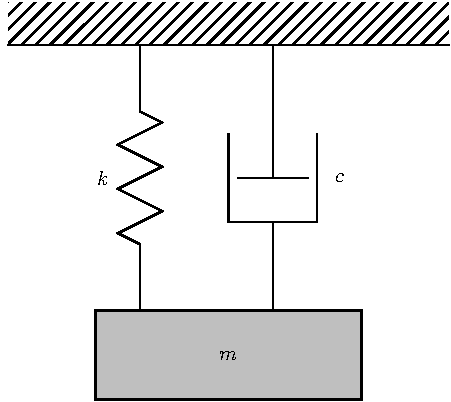
\includegraphics[width=0.4\linewidth]{graphics/notes_08_hanging_mass}

 Write out the DE for the position of the mass, given $F_{\mbox{ext}} = A
 \sin(Bt)$.


\newpage

\problem
  Sketch an RLC circuit, with the voltage supply (or `electromotive
  force') of $\ds E(t) = \frac{-A}{B} \cos(Bt)$, and write out the DE
  for the current in the circuit.

\vfill

What might give rise to an EMF of this form?
\vspace{1in}

\newpage

Comment on the similarity between the mathematical model of the
spring/mass, and of the RLC circuit.

\newpage

\topic{Demonstration - Forced Oscillations}

We will explore the solutions of/predictions for the spring/mass
system (and RLC circuits!) through changing parameters in a
simulation.  We will consider both
\begin{itemize}
\item graphs of the solutions, and 
\item mathematical forms of the solutions.
\end{itemize}

Your job during the demonstrations is to track:
\begin{itemize}
\item the amount of friction,
\item the {\em natural} frequency (in $y_c$), and
\item the {\em stimulating} frequency (in $Fe$ and $y_{NH}$)
\end{itemize}

\newpage

{\bf Unforced Motion}

Setting $F_{\mbox{ext}} = 0$, review the effect of
  increasing the friction coefficient $c$ on the $y_c$ solution.

\vfill

What is the $y_{NH}$ solution for all these simulations, and why?

\vfill

\newpage

{\bf Forced, but Undamped Motion}

Now we turn off the friction (by setting $c=0$) to zero, and
start to apply the external force. \\
We set $F_{\mbox{ext}} = 10 \sin(1.0 t)$.   \\
What is the form of $y_c$, and what is the form of $y_{NH}$?

\vfill

Experiment with the frequency in $\Fe$, in the range 0.5 to 3, or well
above 5.  Does the motion of the mass over time make sense?

\vfill

\newpage

\topic{Demonstration - Resonance and Near-Resonance}

{\bf Resonance}

Set $\Fe = 1 \sin(5t)$.  What is special about the
  frequency 5 rad/s?

\vfill

Describe the graph of the solution.

\vfill

Give the mathematical reasons for the graph of the
  simulation.\\

\vfill

The condition of having the external force at {\em exactly} the same
frequency as the natural vibrations is called {\bf resonance.}  Note:
for true resonance, there must be {\em no friction.}

\newpage

{\bf Near-Resonance}

Admitedly, resonance is a unique event requiring {\bf perfect}
matching of the stimulating force with the natural frequency.

Explore frequencies in $\Fe$ {\em close to} 5.  Describe
  the resulting solutions, both for their amplitude and any other
  response.

\vfill

Give the mathematical reasons for the shape of the graph
  for near-resonance response.

\vfill

Note again that there is {\em no friction} with this response.

\newpage

\topic{Demonstration - Practical Resonance}

{\bf Adding in Friction - Practical Resonsance}

Set $F_{\mbox{ext}} = 1 \sin(5t)$ again, but set friction $c$ to 0.1 Compare this
solution to the one without friction, both graphically and
mathematically.

\vfill

Gradually increase the amount of friction.  Describe how the solution
changes.

\vfill

How is this more realistic than the undamped case?

\vfill

How do the mathematical forms of the pure-resonance (undamped) and
practical resonance (some damping) compare?

\vfill

\newpage

\topic{Transient and Steady-State Solutions}
\subsection*{Transient and Steady-State Solutions}

More generally, when there is friction in the spring/mass system and
an oscillatory external force, we can break the solution into two
parts: {\em transient} and {\em steady state}.

We set $F_{\mbox{ext}} = 1 \sin(t)$, and $c = 1$ for friction, which is fairly
high for an oscillating system.  Describe the resulting behaviour.

\vfill

Specifically, what are the two natural frequencies in the solution?

\vfill

Which frequency is present in the {\bf long run}?

\vfill

\newpage

In a damped physical system with forced oscillations, is $y_{NH}$ {\bf
  transient} or {\bf steady-state}, and why?

\vfill

In a damped physical system, is $y_c$ {\bf transient} or {\bf
  steady-state}, and why?

\vfill

\newpage

Reminder: we study the simple damped spring/mass system in such depth
because
\begin{itemize}
\item the system displays all the interesting mathematical solution
  forms as we vary just a few parameters, 
\item we hope that the simplicity of the system, and its resemblance
  to familiar systems like swings or bouncing a basket ball, help to
  you associate the mathematics with the real-world behaviour.
\item the DE for the spring/mass system is either identical or similar
  to those for a number of other real-world scenarios, like electronic
  circuits.
\end{itemize}


% \newpage
%      Resonance can be good or bad depending on the circumstances.
%        \begin{itemize}
%        \item pushing someone on a swing
%        \item the timekeeping mechanisms of modern clocks and watches,
%          e.g. the balance wheel in a mechanical watch and the quartz
%          crystal in a quartz watch
%        \item acoustic resonances of musical instruments
%        \item failure of the original Tacoma Narrows Bridge 
%        \end{itemize}

% \end{proof}

\newpage

\topic{Analytic solutions to DEs}
\subsection*{Analytic solutions to DEs}
To compute an analytic solution, we must
\begin{itemize}
\item Recognize form of DE 
\vspace{0.5cm}
\item Properly execute solution technique
\vspace{0.5cm}
\item Include ``+C'' at appropriate moment
\vspace{0.5cm}
\item Solve for C using initial conditions
\end{itemize}
Finally get $y(t) = $

\vfill

\newpage

Unfortunately, that can all be a lot of work.  Sometimes, we just want
the prediction of $y$, position, velocity, etc. over time.
\begin{itemize}
\item In {\em principle}, the pair (DE + initial condition) is enough
  to define prediction for all time.
\item The difficulties in finding analytic solutions come from the
  necessary integration/solution step.
\item MATLAB can generate an {\em approximate numerical solution} {\bf
    without} need to integrate!
\end{itemize}

\vfill

\newpage

\subsection*{In MATLAB}
There are two main ingredients to generating a numerical solution/prediction 
from a differential equation:
\begin{itemize}
\item Define the DE as a MATLAB function.
\item In a separate script, pass the DE to a DE solver, along with the
  initial conditions and the desired time span for the simulation.
\end{itemize}

\problem Create a file called \texttt{tempDE.m}, which
computes the derivative based on the DE
$$\frac{dy}{dt} = -k (y - T_{\mbox{ext}})$$

\vsc

Note that the MATLAB function is a {\bf direct implementation} of the
DE formula: you do {\bf not} do any solving at this stage!

\newpage

\subsection*{Generating Numerical Solution}

\problem Search for ``first order ODEs'' or ``initial value problem''
  in MATLAB help.
\vsc 
\vsc 

\problem What form of differential equation does MATLAB assume we have?

\vsc
\vsc


\newpage

Note that differential equation solvers are a big component of MATLAB:
you may have to do some reading to sort out the kind of equation you
have, and what the appropriate solving tool is.

\problem Which of the solvers is recommended as a ``first try'' solver?

\vsc
\vsc

\newpage

\subsection*{ode45}
The first solver to reach for in MATLAB is \verb#ode45#.  To run it, we need
\begin{itemize} 
\item the DE function {\bf in form $\displaystyle \frac{dy}{dt} = f(t, y)$};
\vfill
\item the time span for the solution/simulation, $[t_0, t_{\mbox{end}}]$; and
\vfill
\item the initial condition ($y(t_0))$
\vfill
\end{itemize}

\newpage

\subsection*{Example - Step 1}
The following comes from the script \texttt{W8\_1.m}, on the course
web site.
\begin{verbatim}
% Define temp DE in the form dy/dt = f(t, y)
% and set other constants
k = 0.7;  % /min

T_ext = 20; % external/environment temp

DE = @(t, y) tempDE(y, k, T_ext);

\end{verbatim}

\newpage

\subsection*{Example - Step 2}
\begin{verbatim}
% Solve based on initial condition
y0 = 100;  % initial temperature

time_span = [0, 30];  % interval for solution

[t, y] = ode45(DE, time_span, y0);

plot(t, y);
\end{verbatim}

\newpage

To decipher and work with the output, it is critical that you
understand what MATLAB provides.  
\begin{itemize}
\item The final values of \verb#t# and \verb#y# are 
\vfill
\item \verb#t# starts at
\vfill
\item \verb#t# ends at
\vfill
\item \verb#y# starts at
\vfill
\end{itemize}

\newpage

\subsection*{Basic Process}
How does MATLAB do it?
\vfill
\vfill

\newpage

\subsection*{Example - Pendulum }
\vfill
\begin{align*}
  \mbox{Newton's Second Law: }   m  L^2 \theta'' & = T_g + T_f  \\
  & = - m L g \sin(\theta) - (\mu L^2 m) \theta' \\
  \mbox{Solving for $\theta''$: }\theta'' & = - \frac{g}{L} \sin(\theta) - \mu 
  \theta'
\end{align*}

\problem Recalling your work from your differential equations class,
  turn this single second-order DE into a pair of first-order DEs.

\vfill

\newpage


\subsection*{Generality of 1st Order Systems}

Out of all the techniques you learned in your DE class, this
transformation of higher-order DEs to systems of first-order ones will
be essential for this class:
\begin{center}
MATLAB solvers like \verb#ode45# {\bf only} handle 1st order
  systems of DEs
\end{center}
In practice, this is not a limitation because:

\vfill 

\newpage

\problem Download the representation of this system of DEs,
  \texttt{pendulumDE.m}.  Compare it to our DE system,
\begin{align*}
\frac{d y_1}{dt} & = y_2 \\
\frac{d y_2}{dt} & = -\frac{g}{L}\sin(y_1)  - \mu y_2
\end{align*}
\vsc

\problem Download and run the script \texttt{W8\_2.m}.

\vsc

\problem What were the initial conditions of the pendulum?

\vfill

\problem Based on that information, what do the two curves on the graph
  represent?

\vfill

\newpage

\problem Change the script so the pendulum also has an initial velocity.

\vsc

\problem If we keep the initial angle at $-\frac{\pi}{2}$ (pendulum
  out horizontally), experiment and find the initial velocity that
  will push the pendulum ``over the top''.

\newpage



\newpage

\subsection*{Vector-based Pendulum Model}
We are now going to model the pendulum's motion as if it were free to
move anywhere in space (two full degrees of freedom).  This will
require a more complicated model, but will be more general (i.e. more
like the roller coaster scenario!)

{\bf Free Body Diagram}
The obvious way to determine how the pendulum would move is to
consider all the forces involved.  For now we will just use gravity
and the rod (no friction).

\problem Draw the free body diagram for the pendulum's mass.
\vfill \vfill

\problem Write out $\Fg$ as a force vector.
\vfill

\newpage
The force $\Fr$ is more complicated.

\problem If the pendulum is at the position $(x, y)$, what is the
  {\bf direction} of $\Fr$?

\vfill

\problem What is the {\bf magnitude} of $\Fr$?

\vfill
\vfill

\newpage 

\problem Write out a formula or calculation to determine $\Fr$,
  given the position $(x, y)$.

\vfill

\newpage


\subsection*{Creating the Differential Equations}

\problem Use Newton's Second Law, $ma = \sum F$, to obtain a
  differential equation for $x$ and another for $y$.

\vfill

\newpage

\problem Using the vector $\vec{w} = [x, x', y, y'] = [w_1, w_2,
  w_3, w_4]$ rewrite our second-order system of DEs for $x$ and $y$ as
  a first-order system for $\vec{w} = [w_1, w_2, w_3, w_4]$.

\vfill
\vfill
\vfill

\newpage

\subsection*{In MATLAB}
\problem Download the file \texttt{pendulumXYDE.m}.  Complete it by
  computing the values of $\ds \frac{d\vec{w}}{dt} = \vec{w}'$, based
    on the current state, $\vec{w}$.  You are literally transcribing
    the 1st order DE system we just found into MATLAB.

\vsc

\problem Download and run the script \texttt{W8\_3.m}. 
This script simply sets the initial conditions, the time span
for the simulation, then calls \texttt{ode45} to do the simulating.

\vsc

\problem Fix any errors to get the simulation to run.

\vsc

\newpage

\problem The output of the simulation is a vector \texttt{t} and a
  matrix \texttt{w}.  Sketch them and what their contents mean.

\vfill

\newpage

\problem Add the command we used last class, \texttt{plot(t, w)}, 
to the script and re-run the script. 

\vsc

\problem Interpret the graphs produced.

\vfill

\problem Modify the script so that MATLAB shows the path or
  trajectory of the pendulum over the entire simulation.  Comment on
  the quality of the simulation.

\vfill

\newpage


\newpage

\subsection*{Accuracy}
\verb#ode45# generates a {\em numerical approximation} to the real
trajectory.  As soon as we say ``approximation'', we mean ``there is
error''.  Clearly, the default level of error is unacceptable!

\problem Look up the function \texttt{odeset} in MATLAB Help.  Look
  for the key words like `tolerance' and `error'.

\vsc

\problem In \texttt{W8\_3.m}, replace 
\begin{verbatim}
[t, w] = ode45(DE, [0, t_end], w0);
\end{verbatim}
with
\begin{verbatim}
options = odeset('RelTol', 1e-10)
[t, w] = ode45(DE, [0, t_end], w0, options);
\end{verbatim}

\problem Comment on the change in the quality of the simulation.

\vfill

\newpage

\subsection*{Extension Exercises}

\problem Change the static plot into an animation, showing the
  location of the pendulum, as well as the connecting rod and the axis
  of rotation.

\vfill


\problem Change the initial condition to $(x,y) = (-1, 1)$, above the
  axis of rotation and show the resulting trajectory.

\vsc
\vfill

\problem Add an initial {\bf velocity} of 1 m/s to the model.  Hint:
  in what direction must the initial velocity be for a pendulum? 

\vsc
\vfill

\problem Add a friction force to the differential equations.

\vsc
\vfill

\end{document}


